\section{3D Map preprocessing}

\subsection*{Map sharpening}
As we have indicated before, since map sharpening contributes to increase  signal at medium/high resolution, we recommend to perform this map preprocessing step before tracing the atomic model of cryo-EM  3D maps \citep{ramirez2018}.  To accomplish this task, we are going to use the \scipion protocol able to run an automatic method of local sharpening independent of initial model, based on local resolution estimation  (\scommand{xmipp3 - localdeblur sharpening} \citep{ramirez2018} (Appendix \ref{app:localDeblurSharpening})). Although different algorithms could be used previously to $LocalDeblur$ to compute local resolution, we have selected $MonoRes$ \citep{vilas2018}, implemented in \scipion in the protocol \scommand{xmipp3 - local MonoRes}  (Appendix \ref{app:localMonoRes}).\\ 
Since a map binary mask has to be included as a parameter in this protocol, the first step in the local resolution estimation process will be to build the mask by using the \scipion protocol \scommand{xmipp3 - create 3d mask} (Appendix \ref{app:create3DMask}). Open the protocol form (\ffigure{fig:create3Dmask_1} (1)) and fill in the tap \ttt{Map generation} (2) with the input volume (3) and the density threshold (4). By default, the level value observed in \chimera main  graphics window (\ffigure{fig:chimera_visualization_volume}) \ttt{Tools -> Volume Data -> Volume Viewer -> Level} can be selected as threshold. In the \ttt{Postprocessing} tap (\ffigure{fig:create3Dmask_1} (5)), select \ttt{Yes} in \ttt{Apply morphological operation} (6) and maintain the rest of options by default. 

 
 \begin{figure}[H]
  \centering 
  \captionsetup{width=.7\linewidth} 
  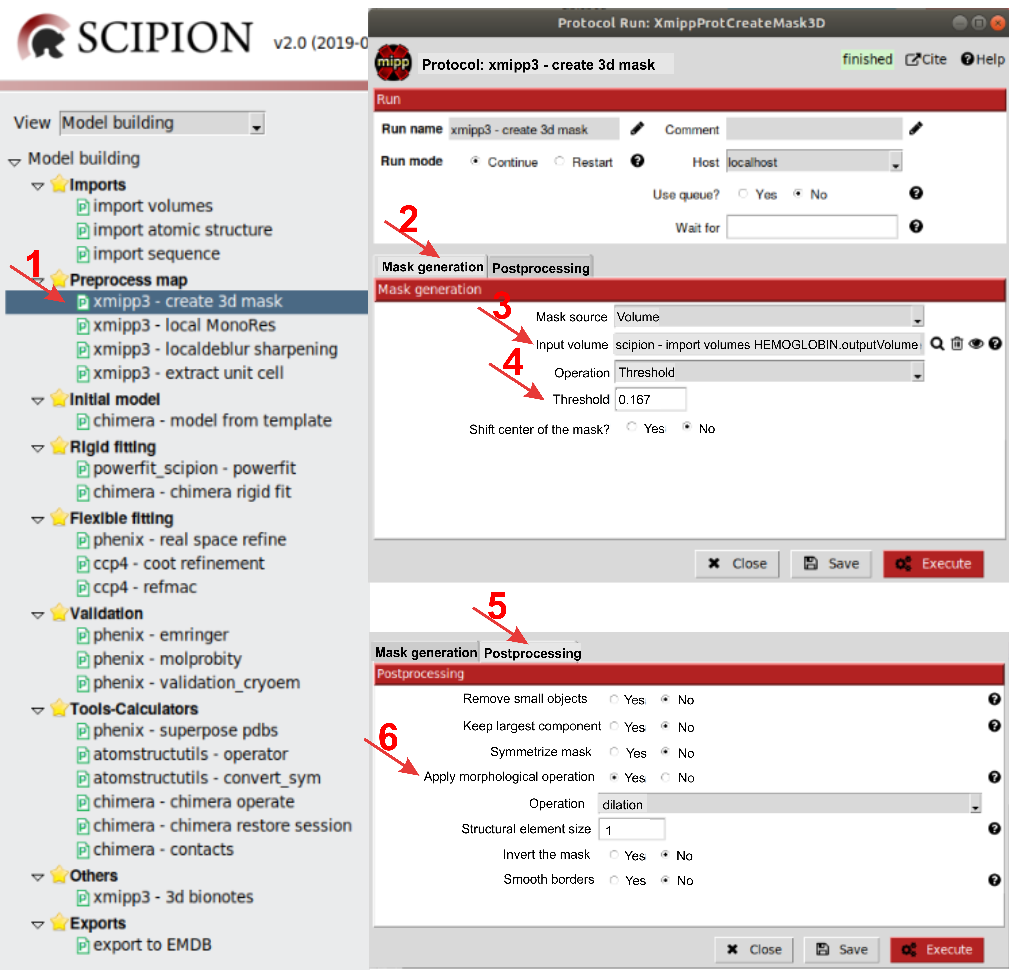
\includegraphics[width=0.80\textwidth]
  {Images/Fig53}
  \caption{Filling in the protocol to create a mask of the initial volume.}
  \label{fig:create3Dmask_1}
  \end{figure}
 
After executing this protocol, the morphology of the mask generated can be checked in slices by clicking \ttt{Analyze Results}. $ShowJ$, the default \scipion viewer, allows visualize the mask with shape similar to the starting volume (\ffigure{fig:create3Dmask_2}).

 \begin{figure}[H]
  \centering 
  \captionsetup{width=.7\linewidth} 
  \includegraphics[width=0.60\textwidth]
  {Images/Fig54}
  \caption{Visualizing the mask of the initial volume.}
  \label{fig:create3Dmask_2}
  \end{figure}
  
Once the mask of the starting map has been created, the protocol of \scommand{xmipp3 - local MonoRes} can be completed to get the estimation of local resolution. Open the protocol (\ffigure{fig:localMonoRes_1} (1)) and include the starting map (2), as well as the binary mask (3). Based on the map resolution (3.2 \AA), select a resolution range between \ttt{0.0} and \ttt{6.0} \AA (4). Finally, get the spherical mask radius (px) (5) previously selected by visual inspection (6) through the wizard on the right.

\begin{figure}[H]
  \centering 
  \captionsetup{width=.7\linewidth} 
  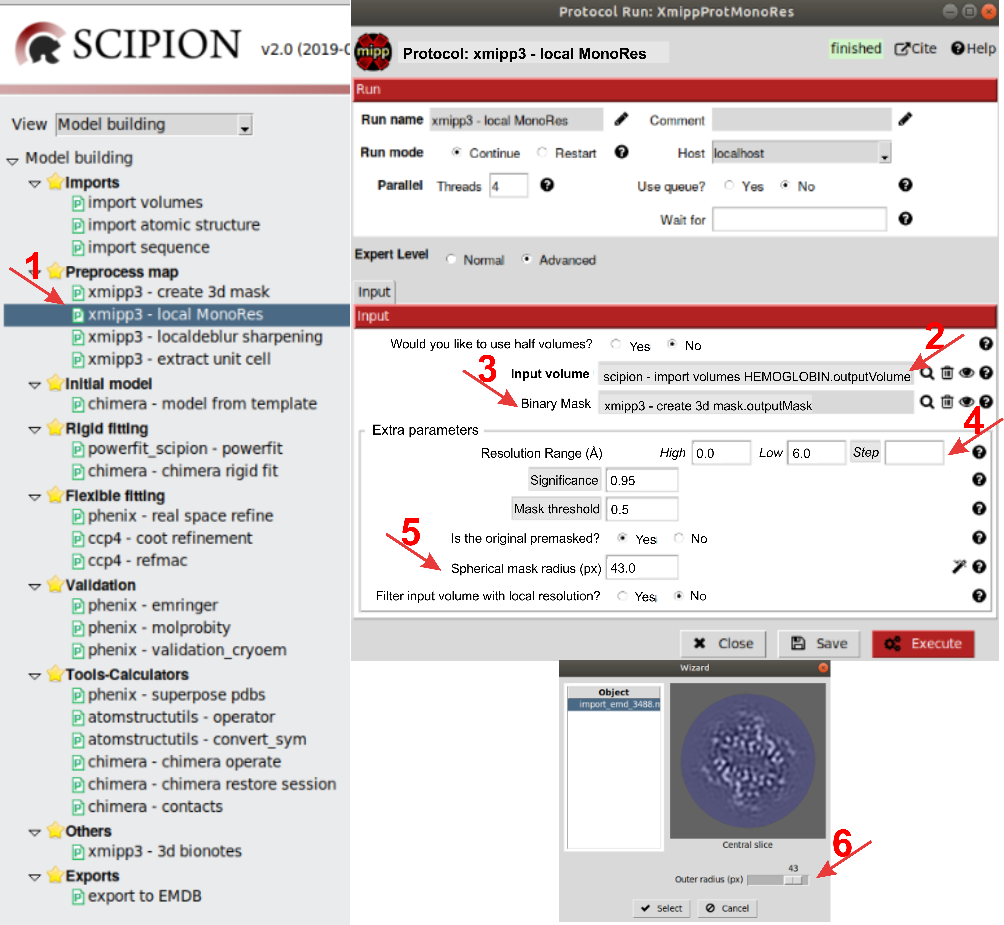
\includegraphics[width=0.80\textwidth]
  {Images/Fig55}
  \caption{Completing the protocol to estimate the local resolution of the \ttt{metHgb} map.}
  \label{fig:localMonoRes_1}
  \end{figure}
  
Execute this protocol and analyze the results. The menu of results (\ffigure{fig:localMonoRes_2} (A)), among other views, shows the histogram of local resolutions (1) and the resolution map in \chimera (2). The histogram of resolutions, which displays the number of map voxels showing a certain resolution, allows to conclude that, although the majority of voxels evidence a resolution between 3.25 and 3.5 \AA, quite close to the published map resolution (3.2 \AA), there are a huge number of voxels displaying higher resolution values, even higher than 6 \AA. The resolution map shown by \chimera details the resolution of each voxel (\ffigure{fig:localMonoRes_3}). The bar on the left indicates the color code for resolution values.

\begin{figure}[H]
  \centering 
  \captionsetup{width=.7\linewidth} 
  \includegraphics[width=0.80\textwidth]
  {Images/Fig56}
  \caption{\scommand{xmipp3 - local MonoRes} menu of results (A) and histogram of resolutions (B).}
  \label{fig:localMonoRes_2}
  \end{figure}
  
\begin{figure}[H]
  \centering 
  \captionsetup{width=.7\linewidth} 
  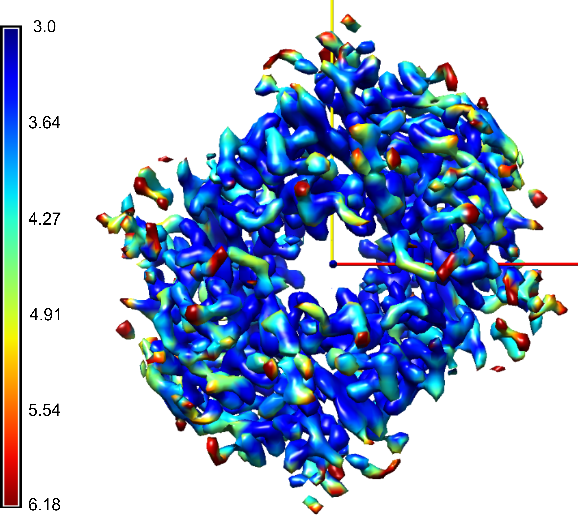
\includegraphics[width=0.70\textwidth]
  {Images/Fig57}
  \caption{Resolution map in \chimera.}
  \label{fig:localMonoRes_3}
  \end{figure}
  
Local resolution values of the input map are used to compute the sharpened map by the \scommand{xmipp3 - localdeblur sharpening} protocol, which implements an iterative steepest descent method that not requires initial model. To accomplish this step, open the protocol (\ffigure{fig:localdeblur_1} (1)) and include the starting map (2) and the map of resolution values (3), maintaining the default values for the rest of parameters (4, 5). 

\begin{figure}[H]
  \centering 
  \captionsetup{width=.7\linewidth} 
  \includegraphics[width=0.80\textwidth]
  {Images/Fig58}
  \caption{Filling in the protocol to compute the sharpened map.}
  \label{fig:localdeblur_1}
  \end{figure}
  
After two iterations, the sharpening algorithm reaches the convergence criterion, \ttt{i.e.} a difference between two successive iterations lower than 1 \%, and stops. The two maps obtained in the respective iterations can be observed with $ShowJ$ by clicking \ttt{Analyze Results} (\ffigure{fig:localdeblur_2}). Visualization in \chimera is also possible selecting ``Open with Chimera'' in the menu option \ttt{File}. The sharpened map obtained after the second iteration will be used in the next step of map preprocessing, the extraction of the unit cell.

\begin{figure}[H]
  \centering 
  \captionsetup{width=.7\linewidth} 
  \includegraphics[width=0.65\textwidth]
  {Images/Fig59}
  \caption{Sharpened maps generated after two iterations.}
  \label{fig:localdeblur_2}
  \end{figure}
  

\subsection*{Extraction of unit cell}
Since smaller volumes usually include lower number of individual structural elements, making easier fitting models in maps and simplifying modeling process, the volume chosen will always be the smaller asymmetrical subunit of the starting loaded volume, also known as unit cell. The size of the unit cell thus depends on the symmetry order of the initial volume. The higher the symmetry order, the smaller the unit cell. The atomic structure of the whole volume will be obtained straight forward by simply repetition of the unit cell structure according to the symmetry. Then, the first step to simplify the complexity of the initial volume is extracting the unit cell. This task can be accomplished by using the \scipion protocol \scommand{xmipp3 - extract unit cell}. 

\ffigure{fig:extract_unit_cell} shows how to fill in this protocol form (1). Since \ttt{metHgb} macromolecule shows symmetry C2, we have selected cyclic symmetry (Cn) as type of symmetry, and 2 as symmetry order. The angle offset selected (-45º) turns around the z axis the mask used to create the unit cell. 
%Remark the relevance of including the offset in order to extract a unit cell able to reconstruct by symmetry the whole volume regarding the symmetry axes. 
The extracted fraction of the initial volume will include the volume comprised between the coordinate origin (inner radius 0.0) and the maximum radius (outer radius 50.0), and will be slightly higher than the unit cell (expand factor 0.2). % We use an expanded unit cell  to favor the modeling of each individual structure edges. 
Again, the respective tutorial appendix \ref{app:extractUnitCell} includes a comprehensive explanation of the meaning of parameters. 

 \begin{figure}[H]
  \centering 
  \captionsetup{width=.7\linewidth} 
  \includegraphics[width=0.90\textwidth]
  {Images/Fig7}
  \caption{Extracting the unit cell volume.}
  \label{fig:extract_unit_cell}
  \end{figure}
  
After executing the protocol (\ffigure{fig:extract_unit_cell}(2)), the resulting expanded unit cell can be observed (3) with \chimera (\ffigure{fig:chimera_visualization_unit_cell}). Note the additional expanded volume of the  unit cell on the left side of the figure. The unit cell itself, on the right side, constitutes the half volume. Since the total volume contains the structure of four proteins, we can predict that this smaller asymmetrical subunit of the initial volume contains two proteins, one $\alpha$ and one $\beta$ \ttt{metHbg} subunits. Then, the respective structures of these two proteins will be fitted in the unit cell volume in successive modeling workflow steps. 
  
 \begin{figure}[H]
  \centering 
  \captionsetup{width=.7\linewidth} 
  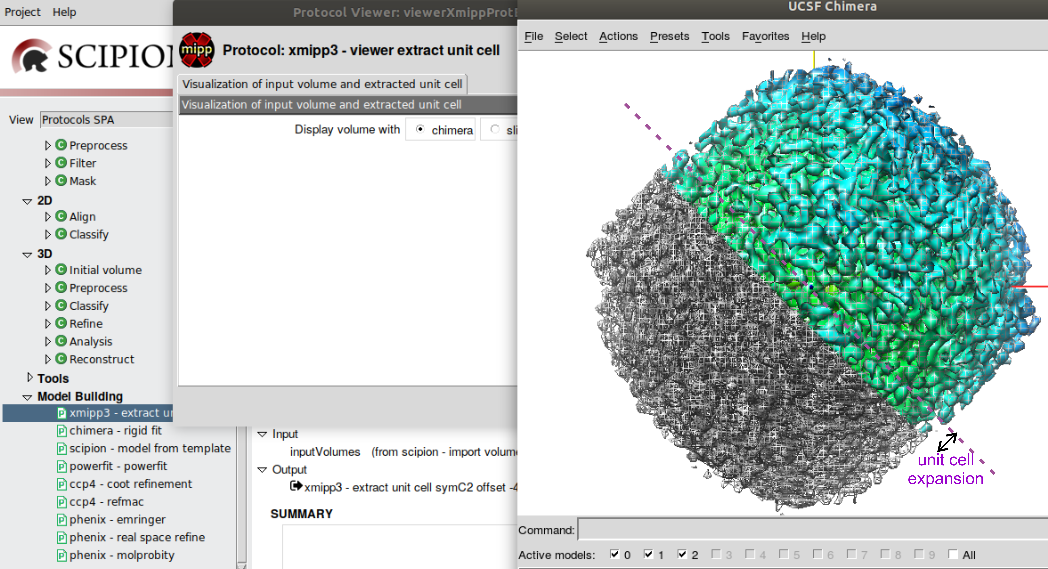
\includegraphics[width=0.80\textwidth]
  {Images/Fig8}
  \caption{Expanded unit cell (green-blue) and initial volume (gray) visualized with $Chimera$. The purple broken line delimits the unit cell (right) and its expanded volume (left).}
  \label{fig:chimera_visualization_unit_cell}
  \end{figure}
